\documentclass[12pt]{beamer}
\setbeamertemplate{navigation symbols}{}
\usetheme{Copenhagen}
\usepackage{listings}
\usepackage{xcolor}
\usepackage{graphicx}
\usepackage{hyperref}
\usepackage{multicol}
\graphicspath{ {imagenes/} }

\definecolor{codegreen}{rgb}{0,0.6,0}
\definecolor{codegray}{rgb}{0.5,0.5,0.5}
\definecolor{codepurple}{rgb}{0.58,0,0.82}
\definecolor{backcolour}{rgb}{0.95,0.95,0.92}

\lstdefinestyle{mystyle}{
    language=c++,
    backgroundcolor=\color{backcolour},   
    commentstyle=\color{codegreen},
    keywordstyle=\color{magenta},
    numberstyle=\tiny\color{codegray},
    stringstyle=\color{codepurple},
    basicstyle=\ttfamily\footnotesize,
    breakatwhitespace=false,         
    breaklines=true,                 
    captionpos=b,                    
    keepspaces=true,                 
    numbers=left,                    
    numbersep=5pt,                  
    showspaces=false,                
    showstringspaces=false,
    showtabs=false,                  
    tabsize=2
}

\lstset{style=mystyle}

\title{Punteros}
\subtitle{Conceptos}
\author{Tomás Peiretti}
\date{}

\begin{document}

\maketitle

\begin{frame}[fragile]{Puntero: definición}
    \begin{columns}
        \begin{column}{0.7\textwidth}
            Un puntero es una \alert{variable que almacena la dirección en memoria} de otra variable. 
            Se dice que los punteros "apuntan a" la variable cuya dirección almacenan. \\
            \medskip
            Si tenemos \textit{int \alert{*} miPuntero;} diremos que \textit{miPuntero} es un puntero que apunta a un entero
            \medskip
\begin{lstlisting}[basicstyle=\scriptsize]
int main() {
    int num = 97;
    int * miPuntero = & num;
    // imprimir la direccion de num:
    cout << miPuntero << endl;
}
\end{lstlisting}
        \end{column}
        \begin{column}{0.3\textwidth}
            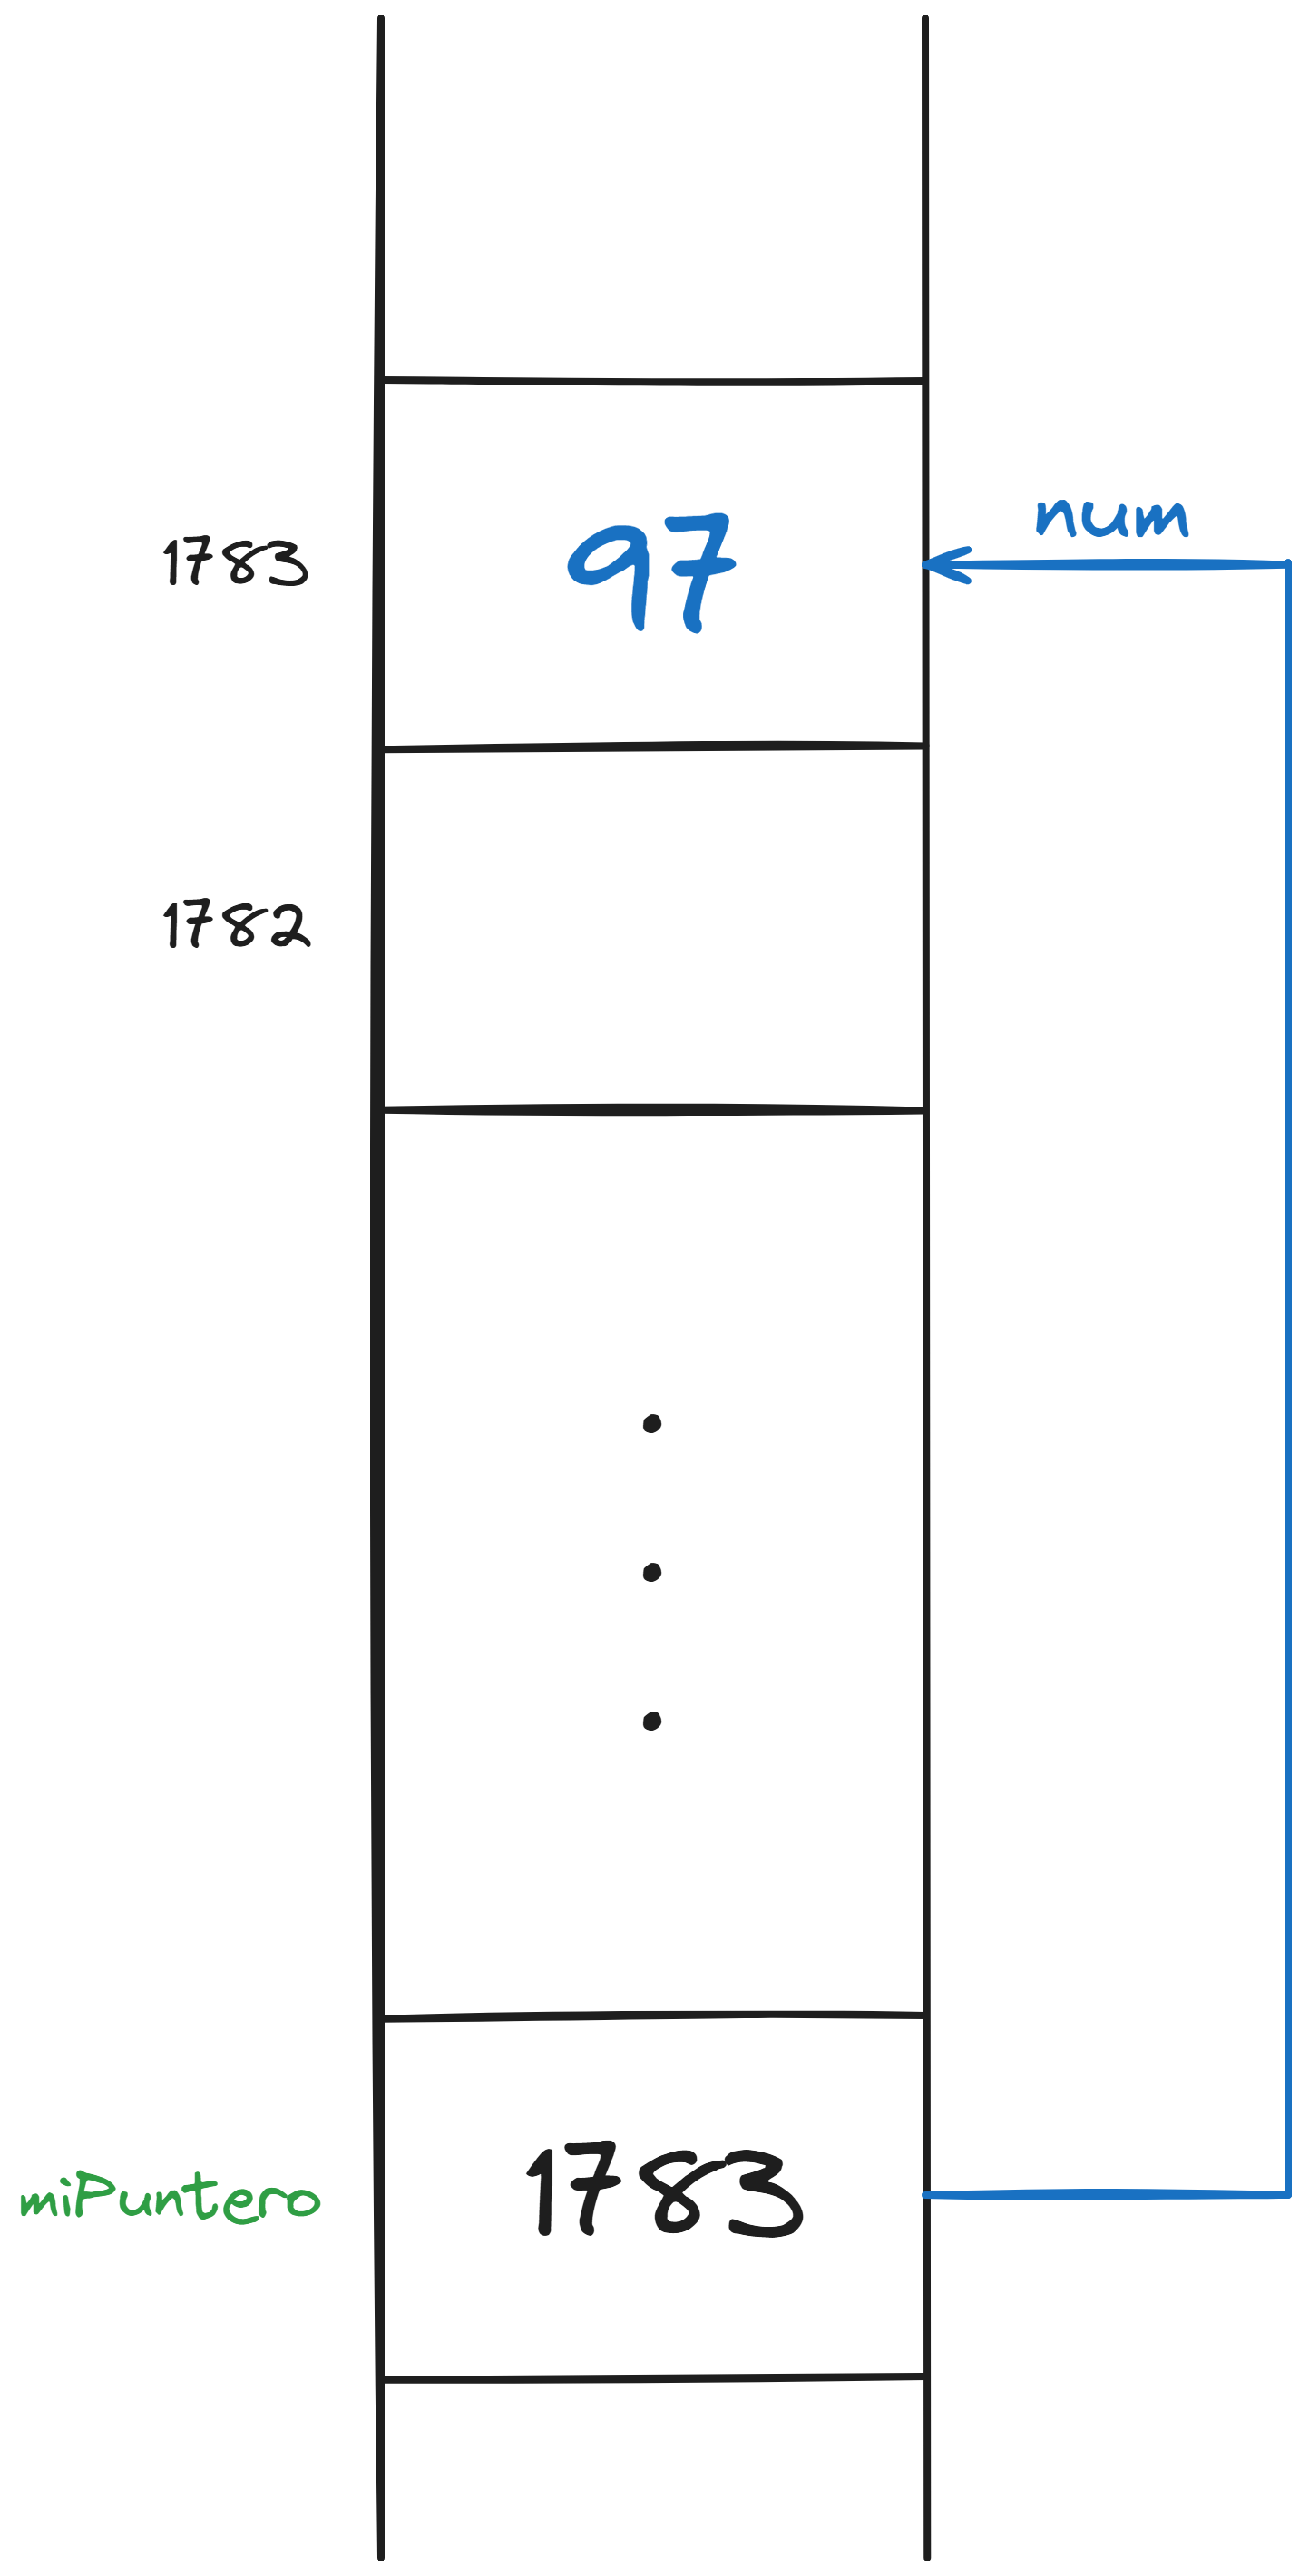
\includegraphics[width=0.8\textwidth]{puntero.png}
            \medskip
            
\includegraphics[width=0.7\textwidth]{puntero_meme.jpg}
        \end{column}
    \end{columns}
\end{frame}

\begin{frame}[fragile]{Punteros: operadores relacionados}
    Para trabajar con punteros, haremos uso de los siguientes operadores:
    \begin{itemize}
        \item Operador \alert{\&}: permite obtener la dirección en memoria de una variable
        \item Operador \alert{*}: permite acceder al valor apuntado por un puntero (de allí su nombre operador de desreferencia)
    \end{itemize}
\begin{lstlisting}[basicstyle=\tiny]
struct Auto {
	string marca;
	int km;
};

int main() {
	int x = 99899;
	Auto mercedes = {"Mercedes", 13526};
	Auto * pAuto = &mercedes;
	
	cout << "el entero " << x << " se encuentra en " << &x << endl;
	cout << "pAuto apunta a " << pAuto << " que es un: " << (*pAuto).marca << endl;
	/* SALIDA:
	   el entero 99899 se encuentra en 0x71ff04
	   pAuto apunta a 0x71fee8 que es un: Mercedes */
}
\end{lstlisting}
\end{frame}

\begin{frame}[fragile]{Operaciones sobre punteros}
    Aparte de los operadores presentados previamente, es posible realizar operaciones de suma y resta sobre los punteros. 
    El comportamiento de estas operaciones varía según el \alert{tamaño del tipo de dato} al que apunten. \\
    \begin{columns}
        \column{0.3\textwidth}\begin{lstlisting}[basicstyle=\tiny]
struct Punto {
    short x;
    short y;
}

int main() {
    char * pChar;
    int * pInt;
    short * pShort;
    Punto * pPunto;
    
    pChar++;
    pInt += 1;
    --pShort;
    pPunto -= 1;
}
\end{lstlisting}
    \column{0.7\textwidth}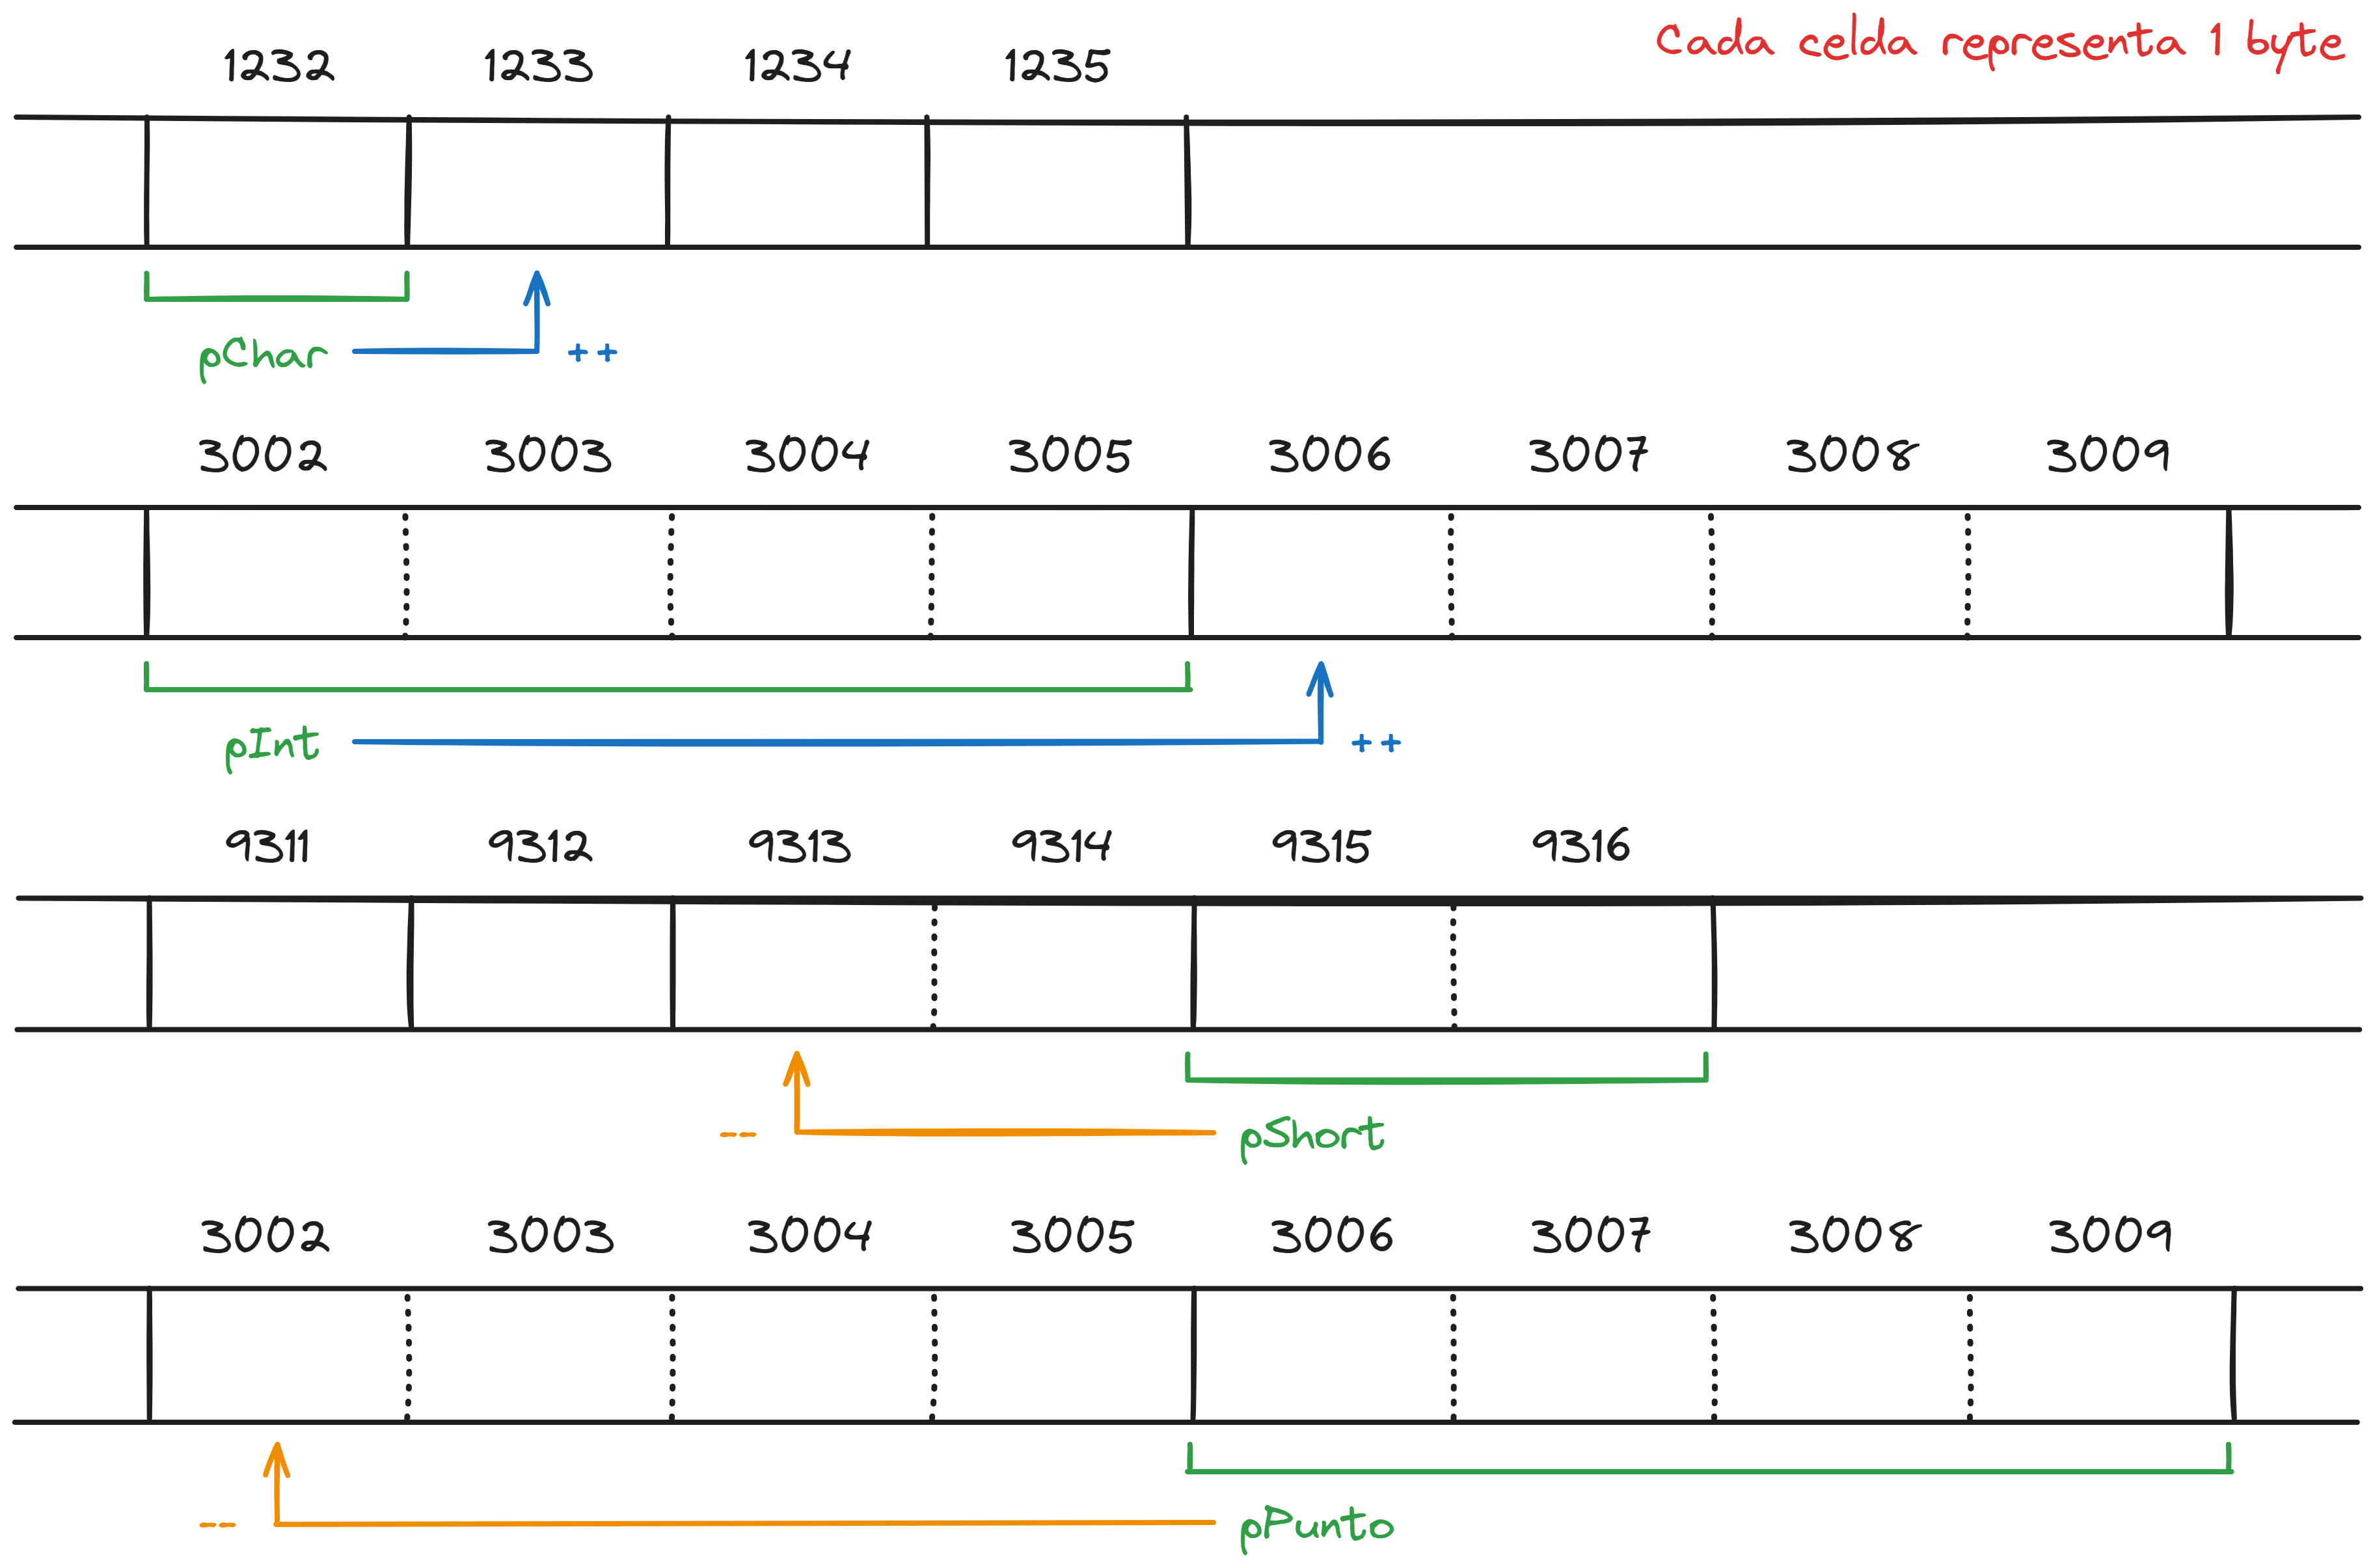
\includegraphics[width=\textwidth]{punteros_suma_resta.png}
    \end{columns}
\end{frame}

\begin{frame}[fragile]{Punteros y arreglos}
\begin{lstlisting}
int main() {
	int arr[5] = {10, 20, 30, 40, 50};
	int * p = arr; // apunta al 1er elemento
	cout << *p << endl; // imprime 10
	
	// *(p+X) === arr[X]
	// actualizar el 3er elemento
	*(p+2) = 9999;
	cout << arr[2] << endl; // imprime 9999
	
	// imprimir el arreglo sin usar []
	for (int * i = arr; i < arr+5 ; i++) {
		cout << *i << " ";
	}
}        
\end{lstlisting}
\end{frame}

\begin{frame}[fragile]{Punteros y structs}
\begin{lstlisting}[basicstyle=\scriptsize]
struct Punto {
    short x;
    short y;
};

// cuando se trabaja con punteros a struct
// es posible utilizar el operador '->'
// para acceder a cada miembro, sin tener que 
// desreferenciar el puntero
int main() {
	Punto p = {10, 5};
	Punto * pPunto = & p;
	
    // en lugar de tener que desreferenciar con *:
    cout << (*pPunto).x << " " << (*pPunto).y << endl;

    // podemos hacer lo siguiente:
    cout << pPunto->x << " " << pPunto->y << endl;

    return 0;
}        
\end{lstlisting}
\end{frame}

\begin{frame}[fragile]{Punteros a punteros}
    C++ permite el uso de punteros que apuntan a punteros que apuntan a datos (o incluso hasta otros punteros). 
    La sintaxis simplemente requiere de un asterisco \alert{*} por cada nivel de indirección:
\begin{lstlisting}
int main() {
    int num = 117;
    int * pNum = &num;
    int ** pp = & pNum;
    int *** ppp = &pp;

    // imprimir num desde p
    cout << **p << endl;
    // Imprimir num desde ppp
    cout << ***ppp << endl; 
}
\end{lstlisting}
\end{frame}

\begin{frame}[fragile]{Punteros a punteros: matrices}
\begin{lstlisting}[basicstyle=\tiny]
const int N = 5;
const int M = 5;

// una matriz implementada con punteros
int main() {
	// arreglo de punteros que apuntan a un arreglo de punteros que apuntan a un entero
	int **m = new int*[N];
	// creacion de la matriz completa
	for (int ** pFila=m; pFila<m+N; pFila++) { 
		*pFila = new int[M];
	}	
	
	// inicializacion de la matriz
	for (int ** pFila=m; pFila<m+N; pFila++) {
		for (int * pCol=*pFila ;pCol<*pFila+M; pCol++) {
			cin >> *pCol;
		}
	}
	
	// impresion de la fila deseada
	int filaAImprimir = 2;
	int * pFila = *(m+filaAImprimir);
	for (int * pCol=pFila ;pCol<pFila+M; pCol++) {
		cout << *pCol << " ";
	}
	
	return 0;
}
\end{lstlisting}
\end{frame}

\begin{frame}{Ejercicios}
    \begin{itemize}
        \item Guía de ejercicios de práctica de la cátedra
        \item Ejercicios del capítulo 12 del libro \textit{C++ para Ingeniería y Ciencias} de Gary J. Bronson.
    \end{itemize}
\end{frame}

\end{document}